\section{Deutsch's Problem}
We wish to explore quantum algorithms and speedups. The first historic example of quantum speedup is from Deutsch's problem. The setup of this problem is as follows. \\
Given $f: \binset \to \binset$, we ask if $f$ is balanced ($f(0) \ne f(1)$) or constant ($f(0) = f(1)$). \\
From here, we give some what we mean by comparing the complexity between classical algorithms and quantum algorithms. \\
For a classical algorithm, we assume $f$ can only be accessed through queries (which is an evaluation of $f$ at a single point), and each query is unit cost. The complexity of the algorithm is the number of queries needed to solve the problem. To solve the above problem with certainty, $2$ queries is needed. \\
For a quantum algorithm, assume we have the ability to apply a $2$-qubit unitary at unit cost, defined by
$$O_f: \ket{\mathbf{x}} \ket{b} \mapsto \ket{\mathbf{x}} \ket{b \oplus f(x)}$$
for all $\mathbf{x}, b \in \binset$. Each application of $O_f$ is a quantum query to $f$. To solve the above problem with certainty, only $1$ quantum query is needed. \\
The quantum circuit is set up as the following:
\begin{center}
    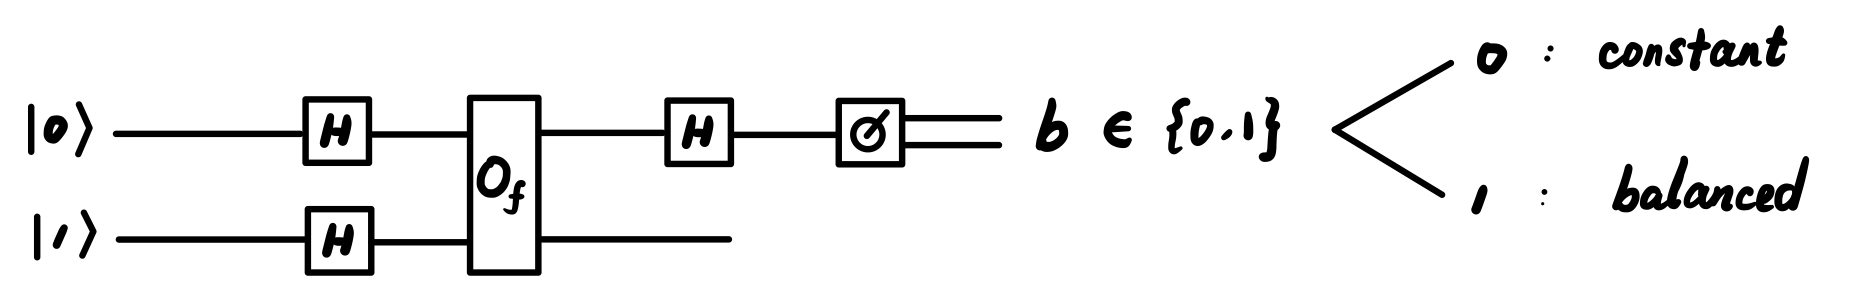
\includegraphics[scale = 0.2]{5/deutsch.png}
\end{center}
During this analysis, two mathetical relations is useful:
$$\ket{0 \oplus x} = \ket{x}$$
$$\ketx - \ket{1 \oplus x} = (-1)^x(\ket{0} - \ket{1})$$
The above circuit, with a single quantum query, can solve Deutsch's problem, the mathematical derivation is not included.
We may also think of this from a partial measurement perspective, where applying a unitary on the non-measured qubit does not change the probability distribution of the measured qubit, so if we apply another Hadamard gate after the quantum query on the second qubit, we can simplify the state before measurement to be:
$$\ket{\psi'} = (-1)^{f(0)} \begin{cases}
    \ket{0} & \text{constant} \\
    \ket{1} & \text{balanced}
\end{cases} \otimes \ket{1}$$

\subsection{Quantum Oracle}
Given $f$ as a classical circuit, we can systematically and efficiently convert a classical circuit diagram into its corresponding quantum oracle.
\begin{definition}
    Let $f: \binset^m \to \binset^n$, the \uimpt{quantum oracle} of $f$ is the unitary matrix $O_f \in \C^{2^{m+n} \times 2^{m + n}}$ defined by
    $$O_f: \ket{\mathbf{x}}\ket{\mathbf{y}} \mapsto \ket{\mathbf{x}}\ket{\mathbf{y} \oplus f(\mathbf{x})}$$
\end{definition}
\begin{theorem}
    Any $f$ can be implemented as a classical circuit involving FANOUT, NOT, AND, OR gates.
\end{theorem}
\begin{theorem}
    Suppose we have the description of classical circuit implementing $f$ in terms of the above gates, we can systematically and efficiently implement $O_f$ using CNOT, X, and Toffoli gates. \\
    More precisely, the implementation takes size that is linear (roughly $2\times$ due to symmetry) in the size (number of gates) of the classical circuit.
\end{theorem}
Specifically, we map FANOUT to CNOT gate, NOT to X gate, AND to Toffoli gate, and OR can be implemented using Toffoli and X gates (because OR can be implemented using NAND gates). An example is the following:
\begin{center}
    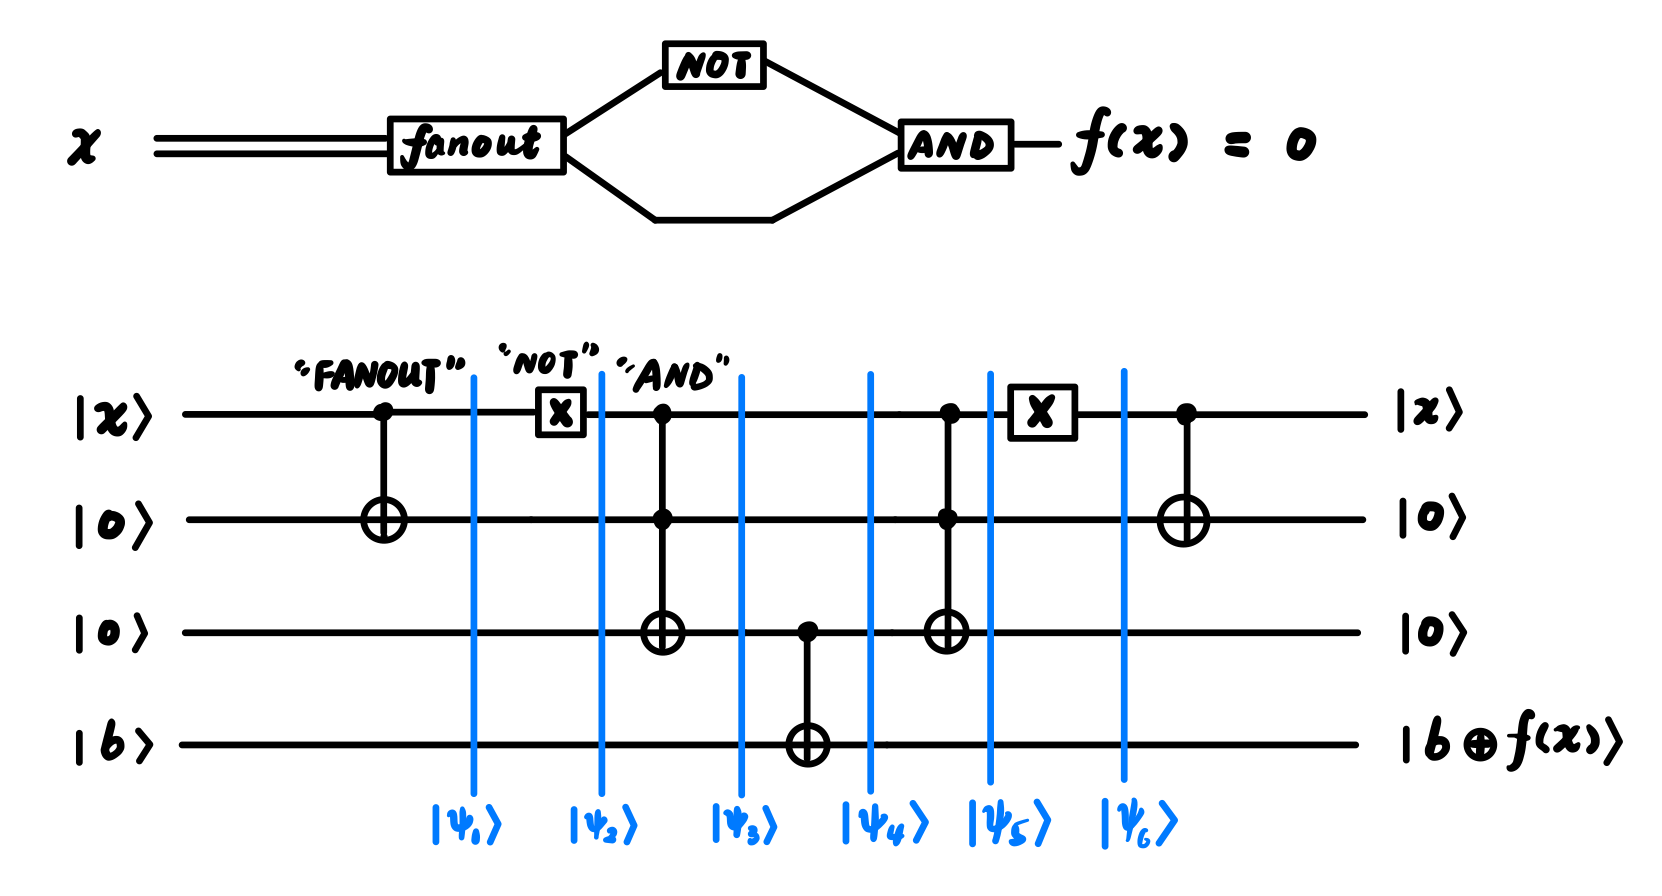
\includegraphics[scale = 0.2]{5/oracle.png}
\end{center}
We can consider CNOT ``copying'' a bit (because $0 \oplus x = x$), X negates a bit (because X maps $\ket{0}$ to $\ket{1}$ and vice versa), Toffoli taking two bits and put the AND result into the third bit (because Toffoli only flips the third bit if both first bit and second bit are $1$).

\newpage